All projects in this dissertation are based on two types of information, 
register data and genotype data. The registers are used to define the study 
population, acquire phenotype information for individuals, and link family 
members. The genotype data is used to run a genome-wide association study (GWAS, See 
\cref{sec:GWAS} for details). This dissertation aims to increase power of a 
GWAS without increasing the sample size of the genotyped data, but instead by 
utilising the additional information available from the registers. 

\subsection{Danish registers}
The Danish registers provide the main source of phenotypic information and allow us to link individuals to their family members. The registers can be linked to one another through a unique 10-digit number assigned to every Dane and resident in Denmark since 1968. In \cref{fig:registerBubbles} is a brief overview of what registers are used and how they are linked together. Details on the mentioned registers will be provided in this section.


\subsubsection{The civil registration system}
The Danish civil registration system was established on 2 April 1968, and all persons living in Denmark were registered for administrative use. All registered individuals were given a 10-digit unique personal identification number, commonly referred to as the CPR-number. The CPR-number is used to link individuals across all registers. This register holds information on gender, date of birth, place of birth, citizenship, identity of parents, and is continually updated with information on vital status, place of residence and spouses. On 1 May 1972 all persons living in Greenland were also included into this register\cite{pedersen2011danish}. 

\subsubsection{The national patient register}
The Danish national patient register was established in 1977. It has been expanded several times since it was created. Originally, it contained only information on patients admitted to somatic wards. In 1995, the register was expanded to also include outpatients, patients from emergency rooms, and patients from psychiatric wards. In 1994, the international classification of disease, version 10 (ICD-10) was adopted in Denmark, and prior to the adoption, ICD-8 was used\cite{lynge2011danish}. 


\subsubsection{The psychiatric central research register}
\begin{wrapfigure}{R}{7cm}
	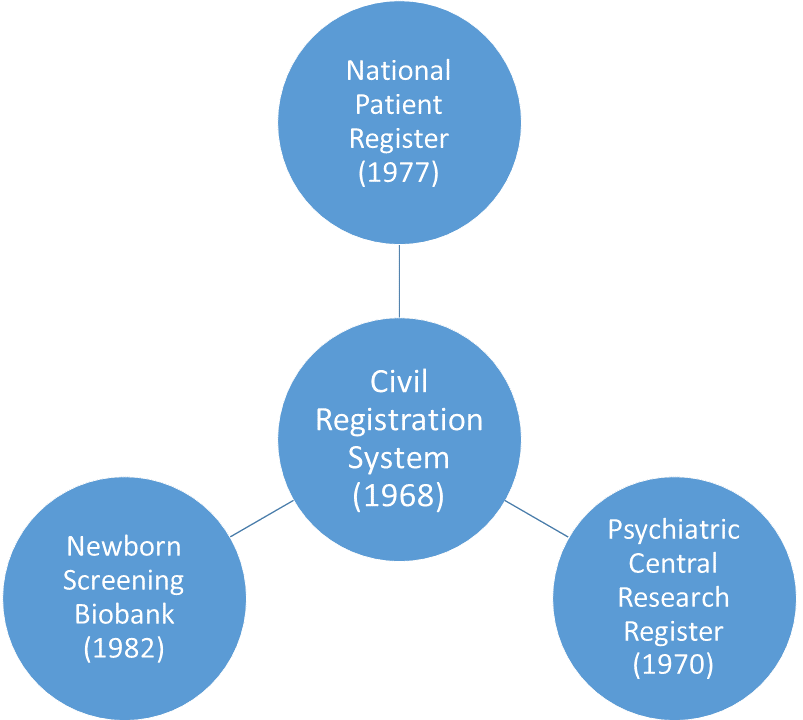
\includegraphics[width=7cm]{intro/registers.png}
	\caption{Illustration of a selected number of Danish registers. They are linked together by the civil registration system. The year denotes the year the register starts.}
	\label{fig:registerBubbles}
\end{wrapfigure}

The psychiatric central research register has valid data from 1970 and onwards. At the beginning, the register contained information on every admission to a mental hospital and psychiatric department, where information such as dates of onset, end of treatment, and all diagnosis were recorded. In 1995, the register became an integrated part of the Danish national patient register and was expanded to also record information from psychiatric emergency room and outpatient treatment. Similar to the national patient register, ICD-10 codes were used after 1995, and ICD-8 were used before. Note that most mild and moderate affected individuals are treated by general practitioners or in private practices, in which case they are not recorded in this register.\cite{mors2011danish}


\subsubsection{The newborn screening biobank}
The Danish newborn screening biobank contains dried blood spot samples from nearly every newborn since 1982. The samples are taken from a heel prick a few days after birth and are stored at $ -20 $\textcelsius. Each year about $ 65,000 $ new samples are added, resulting in over $ 1.8 $ million samples in $ 2007 $. The purpose of the biobank is, among other things, to screen for various diseases at birth. The samples are kept frozen for research purposes, and the dried blood spots provide the basis for the iPSYCH cohort.\cite{norgaard2007storage}.

\subsection{Cumulative incidence proportions} \label{sec:CIPs}
Another important usage for the registers is estimating population representative cumulative incidence proportions(CIPs) that are stratified by sex and birth year. These CIPs will form the basis of how we will account for age of onset. The CIPs have been estimated using the Aalen-Johansen estimator\cite{hansen2017estimating} with death and emigration as competing events. The Aalen-Johansen estimator estimates the survival function when competing events are present. Therefore, it should be used instead of the Kaplan-Meier estimator of the survival function if competing event are present. When stratified by sex and birth year, the CIPs can be interpreted as the proportion of individuals born in a given year and of a given sex who are diagnosed with a phenotype before a point in time $ t $. The data from the registers described above provide the basis for estimating these CIPs and an example of depression CIPs is provided in \cref{fig:CIP_DEP}.


\subsection{Genotype data}
This section covers the sources of genotype data used in this dissertation. There are two main sources, namely iPSYCH and UK biobank (UKBB). Here, we provide a brief overview for both of them. Notably, the iPSYCH cohort is a Danish biobank and has been linked to the previously mentioned registers. 


\subsubsection{iPSYCH}
\begin{wrapfigure}{O}{8cm}
	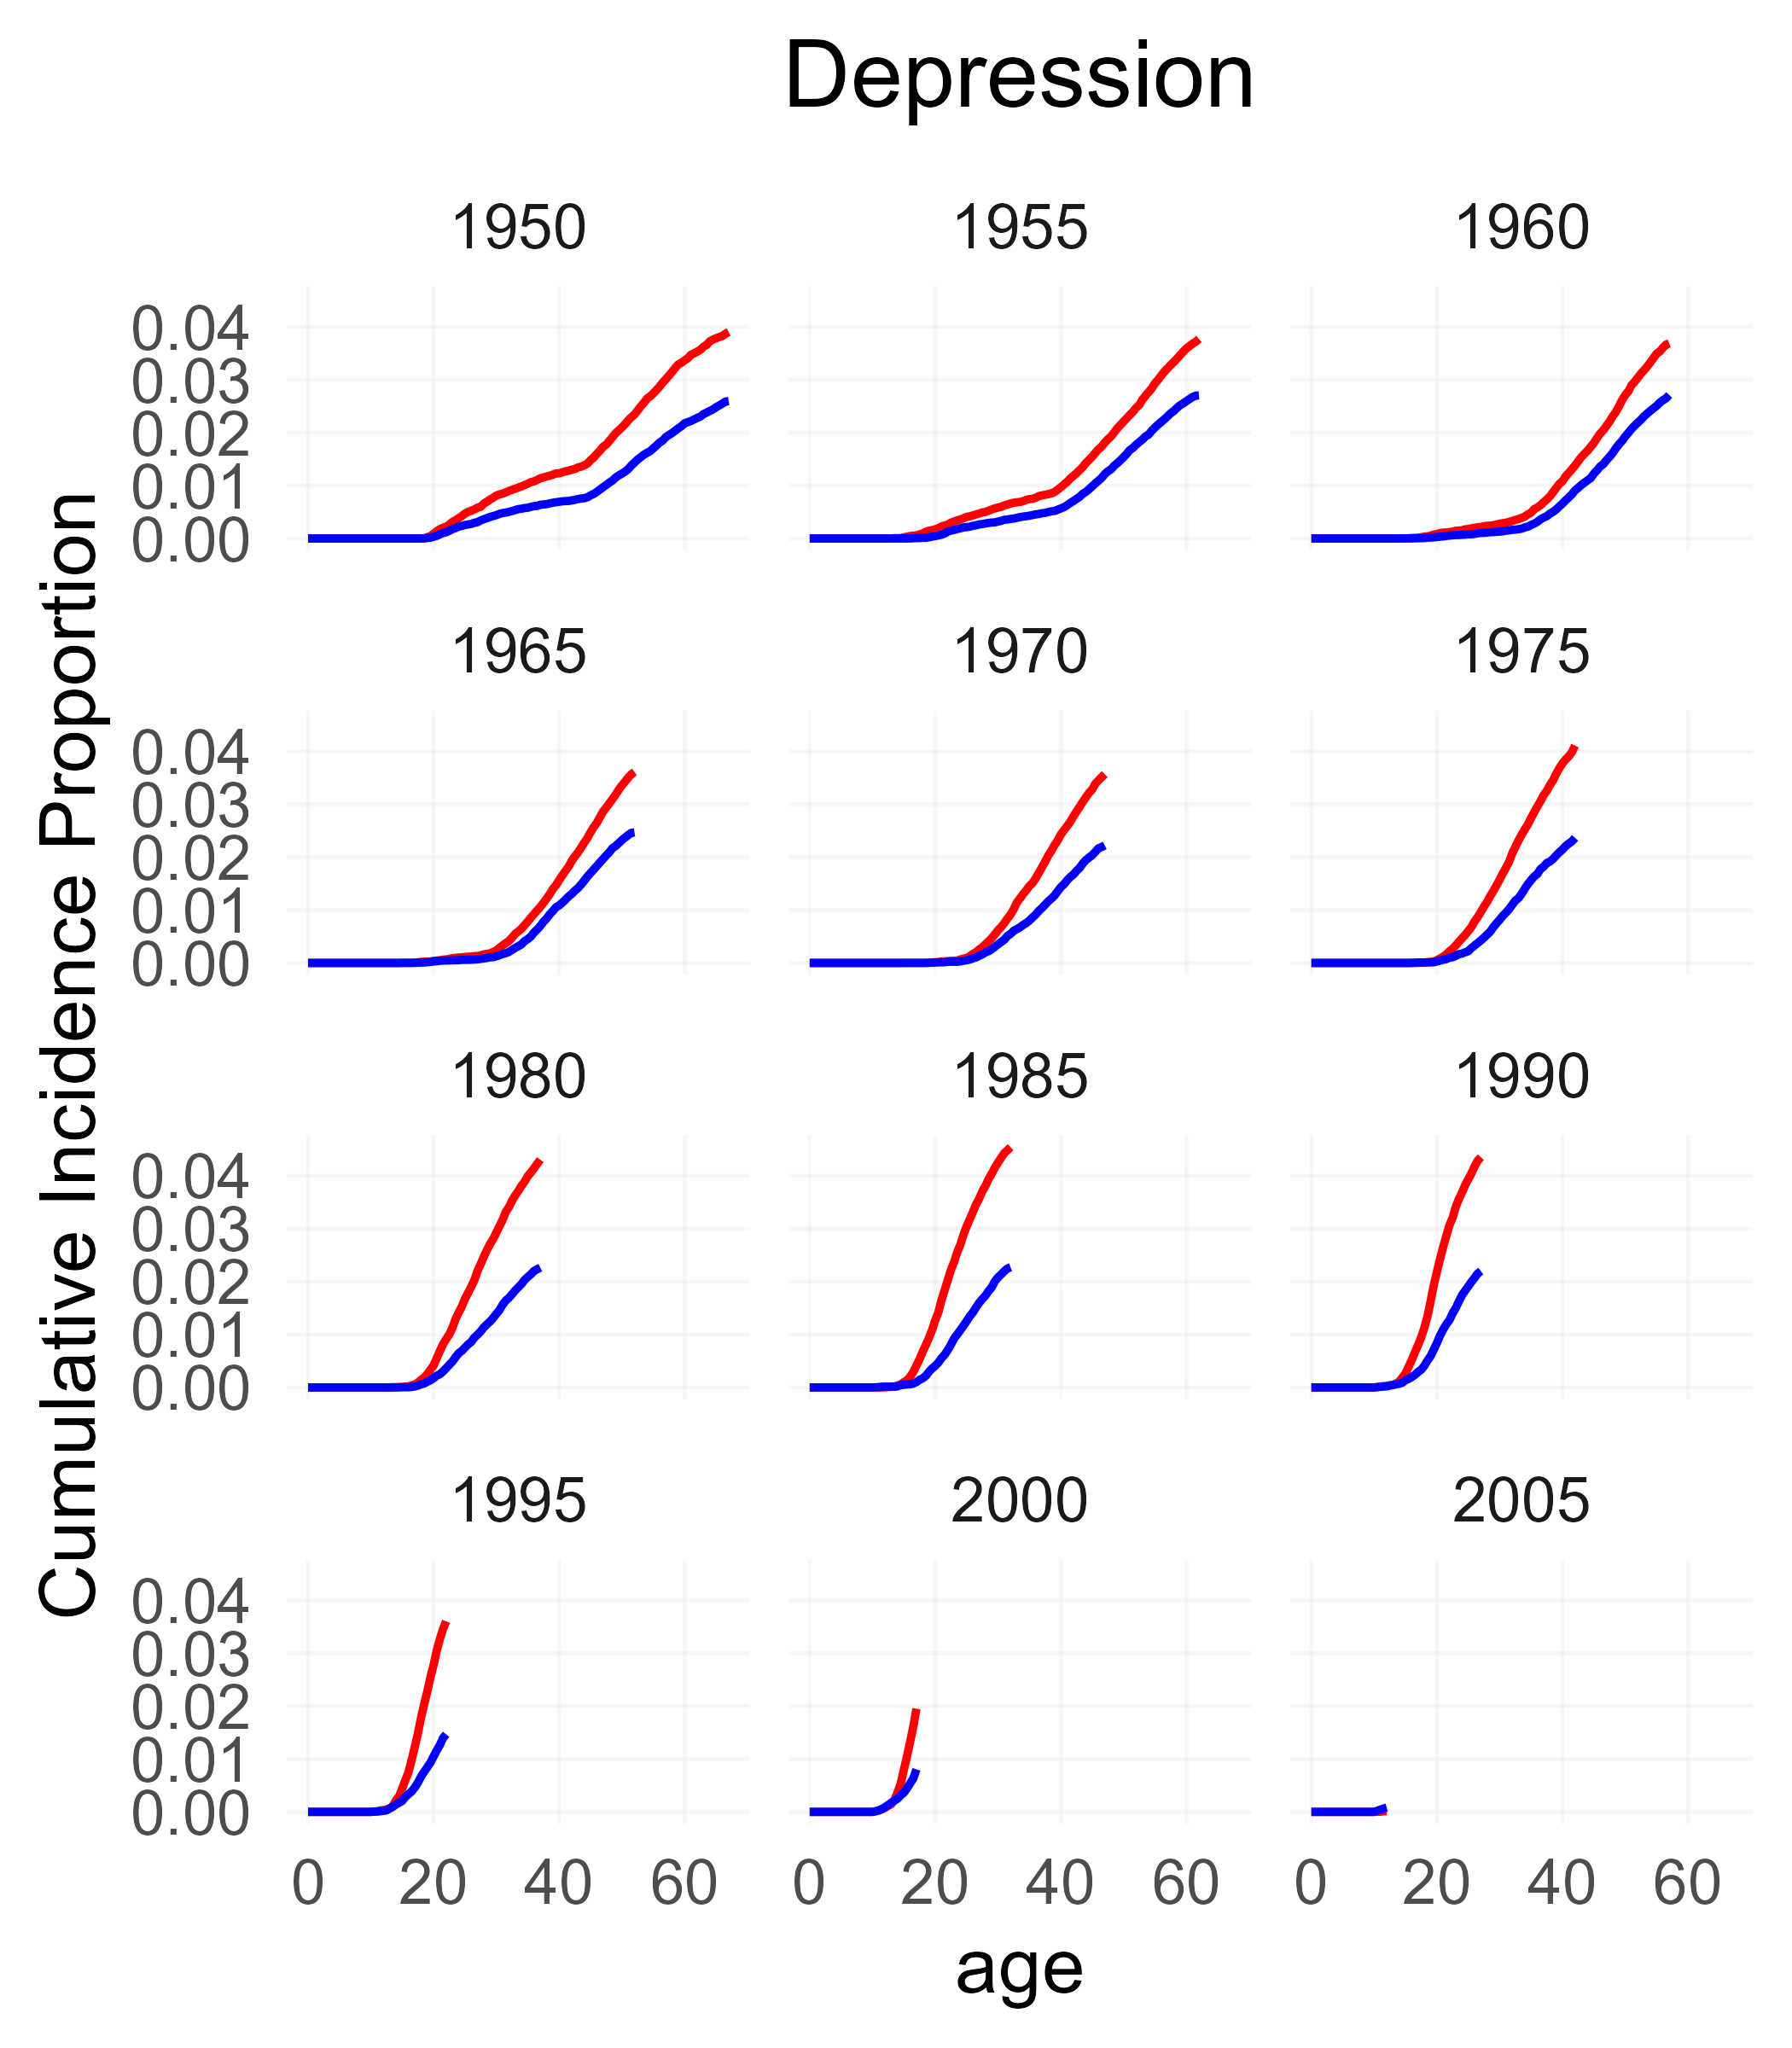
\includegraphics[width=8cm]{methods/prevalencePlot_DEP.png}
	\caption[Cumulative incidence proportions from the Danish 
	Registers]{Depression cumulative incidence proportions estimated from the 
		Danish registers. The CIPs have been stratified by birth year and sex. The 
		red colour represent women and the blue represent men. The CIPs are 
		calculated for each birth year, but are only shown in steps of $ 
		5 $ years.}
	\label{fig:CIP_DEP}
\end{wrapfigure}
source of genotype data used in this dissertation. The benefit of a biobank such as iPSYCH is not the number of genotypes, instead its strength is due to the richness of the register information that it is linked to. All of the previously mentioned Danish registers have been linked to the genotypes, allowing for a very detailed set of phenotypes, as well as multiple information on each individual and their family members. The iPSYCH cohort focuses on psychiatric disorders, namely Attention Deficit Hyperactivity Disorder (ADHD), Autism Spectrum Disorder(ASD), Anorexia Nervosa, Bipolar disorder, Depression, and Schizophrenia\cite{pedersen2018ipsych2012}. Ethical approval was given by the Danish Scientific Ethics Committee, the Danish Health Data Authority, the Danish data protection agency, and the Danish Neonatal Screening Biobank Steering Committee.


The iPSYCH cohort has been sampled in two rounds. The first round is called iPSYCH2012 and has $ 86,189 $ samples, while the second round, iPSYCH2015i, has $ 56,233 $ samples. The combined cohort is called iPSYCH2015 and has $ 141,265 $ unique samples. The population that iPSYCH2012 is nested within is defined as all singletons born in Denmark between the $ 1^{st} $ of May $ 1981 $ and the $ 31^{st} $ of December $ 2005 $, where the mother is known and the child is alive and living in Denmark by their first birthday. iPSYCH2015i extended the study population to individuals born between $ 1^{st} $ of May $ 1981 $ and $ 31^{st} $ of December $ 2008 $ with the same conditions. In total, $ 1,657,449 $ individuals satisfy this condition. For the first round of sampling, $ 30,000 $ samples were chosen at random, creating a population representative control group. For iPSYCH2015i another $ 21,000 $ were sampled for the control group. From the study population, all individuals with at least one of the focus disorders were sampled for iPSYCH2015 resulting in $ 93,608 $ samples, and $ 50,615 $ population controls. However, due to the random sampling $ 385 $ were chosen as controls for both iPSYCH2012 and iPSYCH2015i and another $ 2,958 $ individuals had at least one of the disorders iPSYCH focuses on, and would have been sampled either way. Any recorded case of the disorders of interest for iPSYCH would also be sampled\cite{pedersen2018ipsych2012,bybjerg2020ipsych2015}.

\subsubsection{UK biobank}

It is difficult to overstate the importance of the UK biobank's (UKBB) influence on the field of statistical genetics. Most importantly, UKBB is open access, meaning it is open to researchers from around the world (and not just from the UK), regardless of whether they are from academia, charity, or commercial sectors\cite{bycroft2018uk,biobank2015genotyping}. The biobank is also one of the largest of its kind with about $ 500,000 $ individuals, and it has rich phenotypic information from certain registers, such as cancer and death registers. Some electronic health records have also been linked to the participants, as well as questionnaires on socioeconomic and lifestyle  factors. On top of this information, the participants also provided blood, urine, and saliva samples for proteomic and metabolomic analysis.
%After imputation\cite{marchini2010genotype}, there are roughly $ 96 $ million genetic variants available. After filtering for genetic 
%ancestry (see section \textbf{TODO: REFERENCE ANCESTRY SECTION}), a list of $ 409,728 $ individuals have been released with the data, 
%as these individuals fall in a category with very similar ancestral backgrounds. Relatedness was not recorded during the recruitment 
%process, so relatedness filtering had to be done with kinship coefficients for all pairs of participants. The relatedness analysis 
%showed a larger than expected number of related pairs. The increase is likely due to sampling bias, as samples were taken from 22 
%recruitment centres across the UK, and close living relatives would be more likely to participate if one of them recommended it. 
%\textbf{TODO:Rewrite above section to focus more on family history and age of onset}

The phenotypic information that the UKBB genotypes is linked to is in most cases very detailed. It includes many ICD-9 and ICD-10 codes that participants have been diagnosed with and in some cases even $ when $ they were diagnosed. This allows researchers to perform time-to-event (sometimes referred to as age-of-onset) analysis. However, age-of-onset analysis has so far not achieved the same level of adoption as other types of GWAS analysis such as linear mixed models, but it remains a very popular analysis in fields such as epidemiology\textbf{TODO:ref epi study with surv models}. One reason for the slow adoption of age-of-onset GWAS is likely due to the  computational requirements for such method. Until the publication of SPACox\cite{bi2020fast} and GATE\cite{dey2022efficient}, a proportional hazards model was limited to roughly $ 100,000 $ individuals and other frailty implementations were limited to less than $ 50,000 $ individuals \cite{rizvi2019gwasurvivr,syed2017survivalgwas_sv,he2020fast}. One additional type of information that is not as rich in UKBB is the family history information. In fact, the family history information is only available for $ 12 $ out of thousands of phenotypes. While epidemiology and other fields have utilised family history for a comparatively long time, it is not commonly used in statistical genetics\textbf{TODO: ref studies with FH in other fields. other NCRR papers?}. As an example, family history is one of the risk factors from the framingham heart study \cite{splansky2007third,kannel1990contribution}. Recently, there have been developed some methods that account for family history in some way, such as GWAX, LT-FH, and the method developed in connection with this dissertation, LT-FH++ \cite{gwax,hujoel2020liability,pedersen2022accounting}. It is therefore crucial to continue to link family history, age of onset, and other information from electronic health records to genetic data. 
